\documentclass[aps,onecolumn,twoside,secnumarabic,balancelastpage,amsmath,amssymb,nofootinbib,hyperref=pdftex]{revtex4}


\usepackage{color}         % produces boxes or entire pages with colored backgrounds
\usepackage{graphics}      % standard graphics specifications
\usepackage[pdftex]{graphicx}      % alternative graphics specifications
\usepackage{longtable}     % helps with long table options
\usepackage[english]{babel}
\setlength{\parskip}{1em}
\usepackage{amsmath}
\usepackage{epsf}          % old package handles encapsulated post script issues
\usepackage{bm}            % special 'bold-math' package
\usepackage{verbatim}			% for comment environment
\usepackage[colorlinks=true]{hyperref}  % this package should be added after all others % use as follows: \url{http://web.mit.edu/8.13}                                    
                                  

\begin{document}
\title{}
\author         {Noah Steinberg}
\email          {nastein@umich.edu}
\date{\today}
\affiliation{University of Michigan - Physics}

\maketitle

\section{SU(5) MFV}

Here we adopt a modified minimal flavor violation, where the flavor group of our model is $\mathcal{G}_{f} = SU(3)_{10} \times SU(3)_{\bar{5}}$. Under this group the standard model particles and yukawas transform as follows:

\begin{align}
u^{c},q,e^{c}&(3,1)\\
d^{c},l&(1,3)\\
Y_{u}&(\bar{6},1)\\
Y_{d},Y^{T}_{e}&(\bar{3},\bar{3})\\
\end{align}

In the MFV spirit all higher dimensional standard model operators should be written with insertions of yukawa matrices to make these operators invariant under $\mathcal{G}_{f}$. The four dimension 6 baryon number violating operators can be made invariant to second order in the yukawas with the following wilson coefficients (each term individual term should appear with a coefficient $c_{i}$).

\begin{enumerate}
\item $C^{ijkl}_{qqql} = Y^{ij}_{u}Y^{kl}_{d} + Y^{ik}_{u}Y^{jl}_{d} + Y^{jk}_{u}Y^{il}_{d}$
\item $C^{ijkl}_{duql} = \delta^{il}\delta^{jk} + (Y^{\dagger}_{d})^{ij}Y^{kl}_{u}$
\item $C^{ijkl}_{qque} = \delta^{ik}\delta^{jl} + \delta^{jk}\delta^{il} + Y^{ij}_{u}(Y^{\dagger}_{u})^{kl}$
\item $C^{ijkl}_{duue} = (Y^{\dagger}_{d})^{ij}(Y^{\dagger}_{u})^{kl} + (Y^{\dagger}_{d})^{ik}(Y^{\dagger}_{u})^{jl}$
\end{enumerate}

Note that $\mathcal{O}_{duql}$ and $\mathcal{O}_{qque}$ can be made into flavor singlets with no yukawa insertions. We choose a basis for the yukawas such that $Y_{u} = \text{diag}(\lambda_{u}, \lambda_{c}, \lambda_{t})$ and $Y_{d} = V_{\text{CKM}}\text{diag}(\lambda_{d}, \lambda_{s}, \lambda_{b})$. Only $\mathcal{O}_{qqql}$ and $\mathcal{O}_{duql}$ can contribute to $p\rightarrow K{^+}\bar{\nu}$. Inserting our choice for the yukawa basis, expanding out the flavor indices, and working to lowest order these two operators contribute to $p\rightarrow K{^+}\bar{\nu}$ as:

\begin{enumerate}
\item $\mathcal{O}_{duql}|_{p\rightarrow K^{+}\bar{\nu}} = -(\bar{s}^{c}_{R}u_{R})(\bar{d}^{c}_{L}\nu_{\mu L})$

\item $\begin{aligned}[t] \mathcal{O}_{qqql}|_{p\rightarrow K^{+}\bar{\nu}} = &V^{2l}\lambda_{u}\lambda_{s}(\bar{s}^{c}_{L}d_{L})(\bar{u}^{c}_{L}
\nu_{l L}) - V^{2l}\lambda_{u}\lambda_{s}(\bar{s}^{c}_{L}u_{L})(\bar{d}^{c}_{L}\nu_{l L}) + \\
&V^{2l}\lambda_{u}\lambda_{s}(\bar{d}^{c}_{L}s_{L})(\bar{u}^{c}_{L}\nu_{l L} - V^{2l}\lambda_{u}\lambda_{s}(\bar{d}^{c}_{L}u_{L})(\bar{s}^{c}_{L}\nu_{l L})
\end{aligned}$
\end{enumerate}

where for $\mathcal{O}_{qqql}$ the neutrino flavor is summed over. We see that $\mathcal{O}_{duql}$ is unsuppressed by the small quark yukawas and CKM angles and will thus dominate over $\mathcal{O}_{qqql}$. With the above, we can compute the $p\rightarrow K{^+}\bar{\nu}$ lifetime by running each of the wilson coefficients for each operator and the yukawa terms down to $\mu = 2\text{GeV}$. There are 5 arbitrary wilson coefficients, and each operator is suppressed by a mass scale $\frac{1}{\Lambda^{2}}$ ($\Lambda$ can be interpreted as the geometric mean of the SUSY breaking scale and the GUT scale). We write the lifetime as a function of these wilson coefficients at $\mu = M_{z}$ and multiply them by the appropriate long range renormalization factors. We extract the fermion masses at $\mu = 2\text{GeV}$ from \cite{quark_masses} and set $\lambda_{i}(2\text{GeV}) = \frac{m_{i}(2\text{GeV})}{2^{1/2}v}$, where $v$ is the Higgs vev.

Below we plot the proton lifetime in this channel for $\mathcal{O}(1)}$ wilson coefficients at $\mu = M_{z}$ vs $\Lambda$, and also as a function of the wilson coefficeints at several different values of $\Lambda$.

\begin{figure}[htbp]
\begin{center}
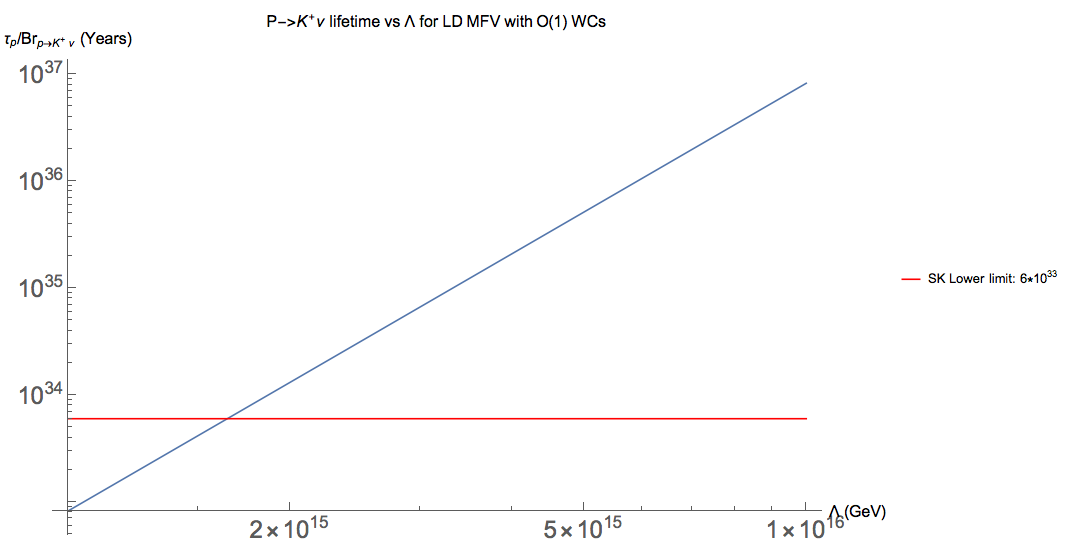
\includegraphics[width=12cm]{lambdas.png}
\caption{$\tau_{p\rightarrow K^{+}\bar{\nu}}$/years for $\mathcal{O}(1)$ wilson coefficients at $\mu = M_{z}$ vs $\Lambda/GeV$. The current lower limit on the lifetime of this channel is $6\times 10^{33}$ years, set by SuperK as of 2014.}
\label{default}
\end{center}
\end{figure}

\begin{figure}[htbp]
\begin{center}
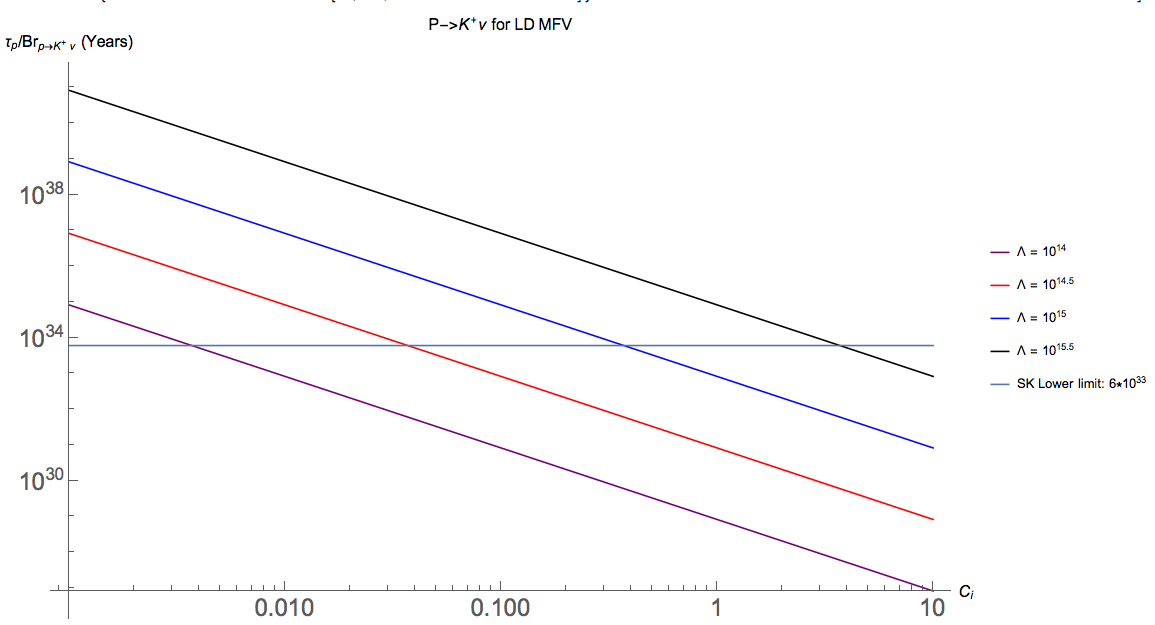
\includegraphics[width=12cm]{wilsons.png}
\caption{$\tau_{p\rightarrow K^{+}\bar{\nu}}$/years for $\Lambda = 10^{14},10^{14.5},10^{15},10^{15.5} GeV$ vs wilson coefficients at $\mu = M_{z}$. The current lower limit on the lifetime of this channel is $6\times 10^{33}$ years, set by SuperK as of 2014.}
\label{default}
\end{center}
\end{figure}

\begin{thebibliography}{9}

\bibitem{quark_masses}
Zhi-zhong Xing et al., "Impacts of the Higgs mass on vacuum stability, running fermion masses, and two-body Higgs decays", Phys. Rev. D 86, 013013 (2012).

\end{thebibliography}


\end{document}